\newpage
\section{\MakeUppercase{Result and Analysis}}
	
\subsection{ASR}
\subsubsection{Word Error Rate (WER) Comparison and Analysis in FastConformer}
\begin{figure}[H]
	\centering
	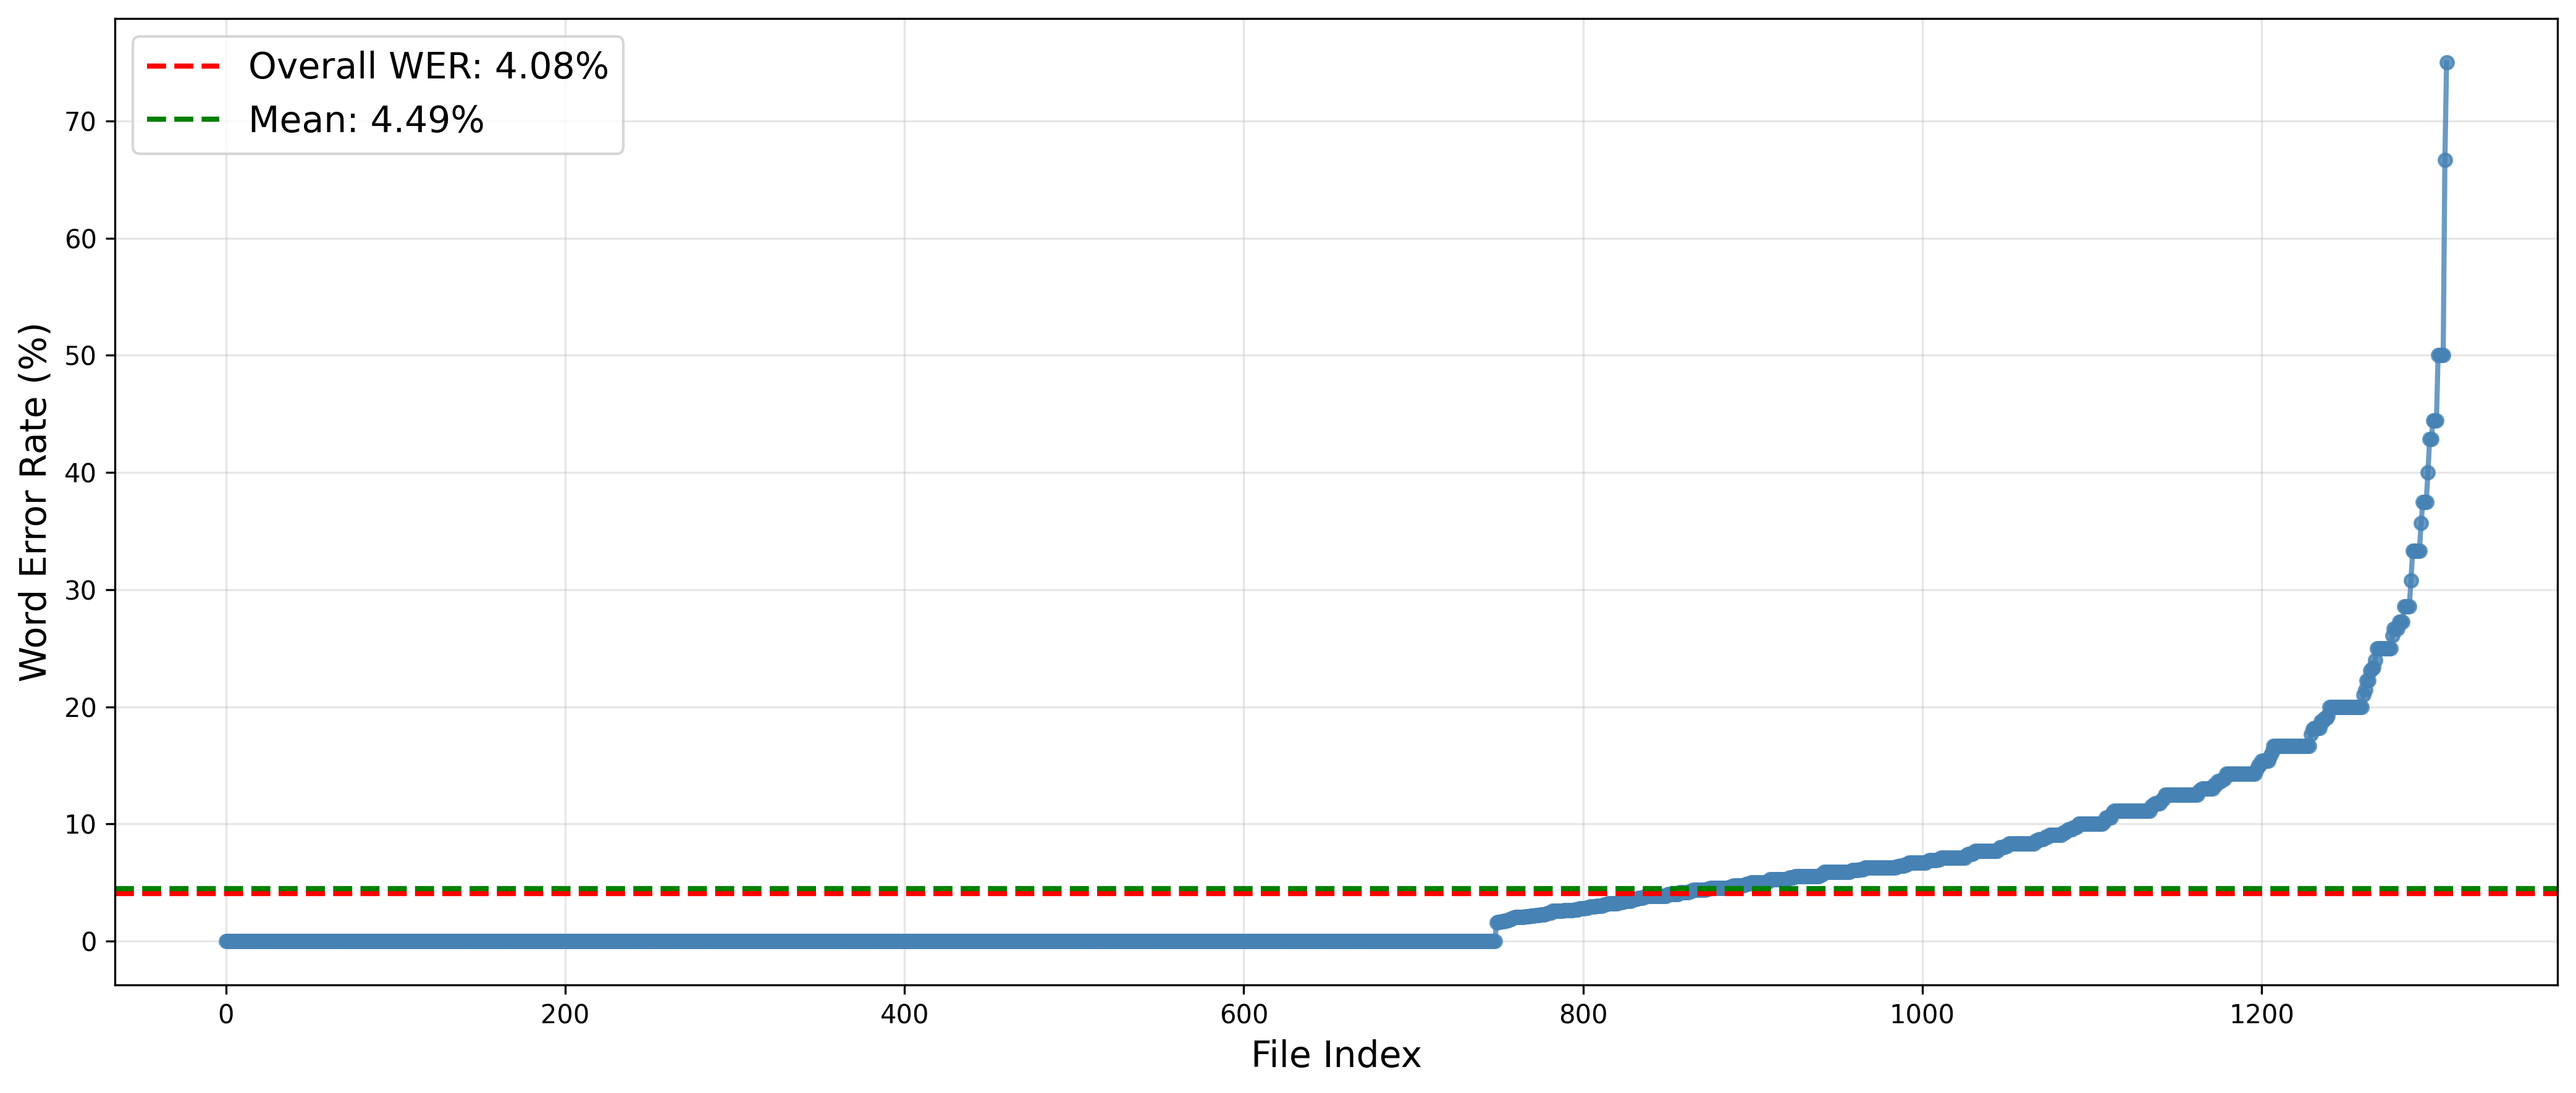
\includegraphics[width=\linewidth]{Images/ASR/Results/shaswot-graphs/WER_LibriSpeech.png}
	\caption{WER on LibriSpeech}
\end{figure}

\begin{table}[H]
	\centering
	\begin{tabular}{|l|c|c|}
		\hline
		\textbf{Model} & \textbf{WER} & \textbf{Parameters} \\
		\hline
		Deep Speech 2 & 5.33 & 110M \\
		Gated ConvNets & 4.8 & 100M \\
		Seq-to-Seq Attention (LSTM Based) & 3.82 & 50M--100M \\
		Convolution Speech Recognition & 3.26 & 30M--70M \\
		wav2vec-wav2letter & 2.7 & 30M / 50M \\
		Transformer & 2.6 & 60M--100M \\
		Squeezeformer (L) & 2.47 & 50M \\
		LSTM Transducer & 2.23 & 40M--80M \\
		Conformer (M) & 2.0 & 50M \\
		Stateformer & 1.76 & 40M--60M \\
		\textbf{Fast Conformer} & \textbf{6.14} & \textbf{13.2M} \\
		\hline
	\end{tabular}
	\caption{Word Error Rate (WER) and parameter count of models trained on the LibriSpeech dataset}
	\label{tab:wer_librispeech_models}
\end{table}
The fine-tuned model has only 13.2 million parameters, which is about 4x to 8x times fewer than smaller architectures (e.g., Conformer-M, ~50 million parameters) and larger ones (e.g., DeepSpeech 2, ~110 million parameters). This compactness makes the architecture very compatible with edge devices and low-latency applications. The encoder is 98.6\% of the total number of parameters, meaning that it washes up all the model capacity, the decoder is insignificant, consisting of only 181K  parameters. This distribution is consistent with CTC based structures that avoid the use of complicated auto-regressive decoders, which limit both memory size and inference complexity.

The achieved WER of 6.14\% per cent is higher than the performance of higher-ranking models, most of which use three to eight times the number of parameters and large amounts of data augmentation, nevertheless, it is a strong performance-per-parameter trade-off. In the case of a situation where constraints in model size, power consumption, or real-time response are involved, the existing model provides a realistically compromised state. The use of a CTC-BPE hybrid output scheme avoids the use of outside language models during decoding, which simplifying the scheme, rather than the many transducer or attention-based models, retains a reasonable degree of sub-word level generalization.

The WER of the model can be further improved to 4.08\% when using greedy decoding, a relatively inexpensive method of choosing the most likely token at each iteration without using a beam search or outside language model rescoring. The only difference is that this can be seen in the red dashed line (Overall WER: 4.08\%), much lower than the green dashed line that shows the average WER (4.49\%), across utterances, shows that not only does greedy decoding increase average accuracy, but also makes performance less varied. This finding highlights the strength of the CTC-BPE hybrid output layer: it is simple with limited decoder footprint, but it produces highly competitive transcription quality, particularly when the factors of inference constraints are important and marginal gains in complex modes of decoding are traded in at the cost of latency and compute efficiency.

\subsubsection{WER, CER and Size Analysis of IndicConformer}
 
\begin{table}[H]
\centering
\begin{tabular}{|l|r|r|}
\hline
\textbf{Model} & \textbf{Parameters} & \textbf{WER (\%)} \\
\hline
Whisper Tiny & 39M & 101.8 \\
Whisper Base & 74M & 102.4 \\
Whisper Small & 244M & 69.5 \\
Whisper Medium & 769M & 54.4 \\
IndicConformer finetuned & 129M & 31.40 \\
\hline
\end{tabular}
\caption{WER (\%) on Clean Fleurs Test Set}
\label{tab:clean_wer}
\end{table}
The clean Fleurs test set results demonstrate that there is a clear comparison of the various Whisper models and the fine-tuned IndicConformer model. Although the models of Whisper get better as they get larger, as Whisper Tiny and Base have very bad WER of 100 and above and 69.5 and 54.4 percent, they are still 10 times worse than the model of IndicConformer that was finetuned. Although it has less parameters (129M), the fine-tuned IndicConformer shows a much lower WER of 31.40\%. This comparison indicates that the IndicConformer fine-tuned model is more effective than all variants of Whisper, which emphasizes that fine-tuning and architecture design play a greater role in the model rather than adding more size to it.

\begin{table}[H]
\centering
\footnotesize
\setlength{\tabcolsep}{5pt}
\begin{tabular}{|l|l|c|c|c|c|c|}
\hline
\rule{0pt}{3ex}\textbf{Model} & \textbf{Type} & \textbf{Size} & \textbf{CER} & \textbf{WER} & \textbf{\shortstack{Global \\[2pt] CER}} & \textbf{\shortstack{Global \\[2pt] WER}} \\
\hline
IndicConformer & NeMo (original) & 493.05 & 15.03 & 35.59 & 13.35 & 33.88 \\
IndicConformer & NeMo (finetuned) & 493.05 & 14.24 & 33.75 & 13.27 & 32.55 \\
IndicConformer & ONNX (full) & 470.22 & 14.24 & 33.75 & 13.88 & 32.49 \\
IndicConformer & ONNX (quantized) & 133.94 & 16.08 & 37.96 & 15.01 & 36.77 \\
\hline
\end{tabular}
\caption{Accuracy Metrics on Noisy Fleurs Test Set}
\label{tab:noisy_accuracy}
\end{table}

The table compares the performance in noisy environments, which gives the character error rate (CER) and word error rate (WER) and global measures. The original NeMo IndicConformer has a CER of 15.03\% and WER of 35.59\%. Once finetuned, the model becomes significantly better: CER declines to 14.24\% and WER declines to 33.75, indicating that finetuning is not only helpful in improving clean speech, but also enhances noise resistance. The trend of global measures is similar, as global CER has decreased to 13.27\% and global WER to 33.55\%, which means that all measures gain continuously throughout the whole data range.

The ONNX full model has the same CER and WER as the finetuned NeMo model with a slight reduction of the model size to 470.22 MB. The ONNX quantized model which is optimized to run at 133.94 MB only, experiences a slight degradation: CER increases to 16.08\% and WER to 37.96\%, with global CER/WER also on the rise, a classic trade-off between model size and accuracy.

\subsubsection{Qualitative Analysis}
To illustrate examples of model predictions on held-out utterances, below there are three representative samples, each paired with its ground-truth reference, the model’s hypothesis, and the corresponding Word Error Rate (WER):

These examples demonstrate that the model accurately captures most of the semantic content. Errors are primarily lexical (e.g., “latter” vs. “latter day”, “to day” vs. “today”) or morphological, which are common in CTC-based systems without external language models. Notably, the model achieves perfect transcription on complex formal language in the second example, highlighting its robustness on well-articulated speech

\subsubsection{Training Dynamics}
\begin{figure}[H]
	\centering
	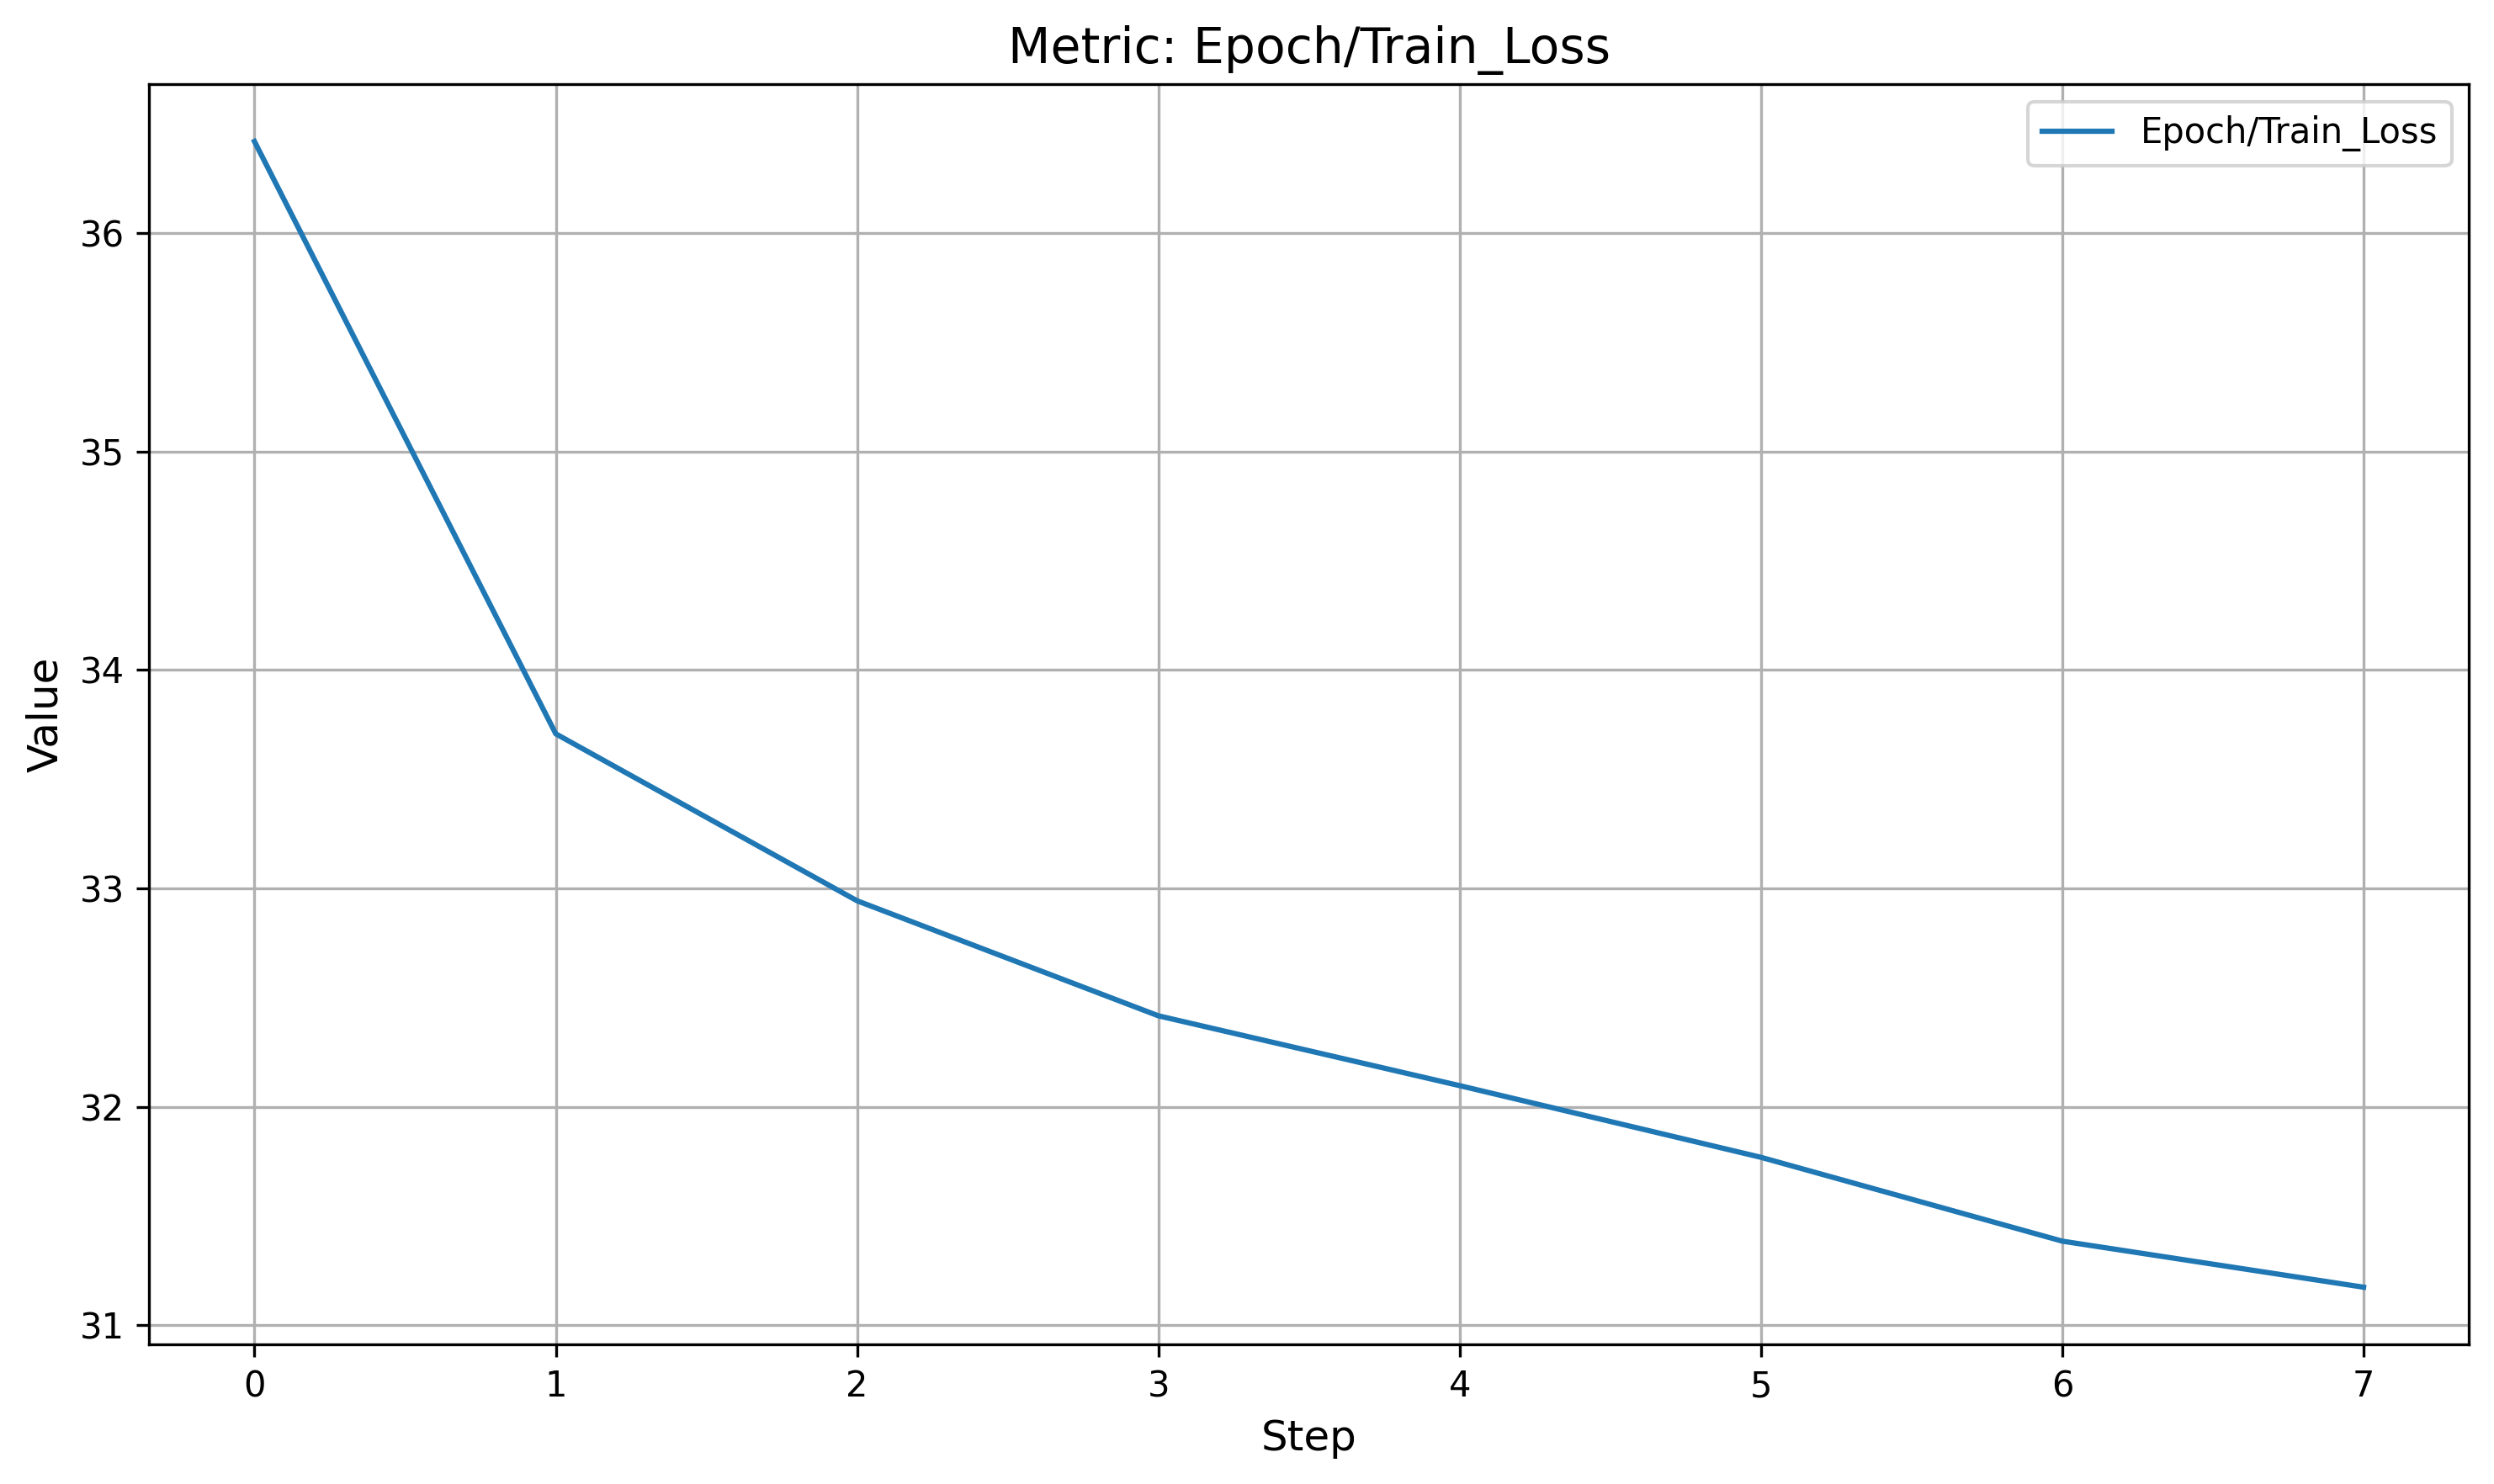
\includegraphics[width=\linewidth]{Images/ASR/Results/shaswot-graphs/EpochTrain_Loss.png}
	\caption{Epoch-wise Training Loss}
\end{figure}

Training Loss (Figure 6-1) decreases steadily from 36.2 to 31.2, indicating consistent learning.

\begin{figure}[H]
	\centering
	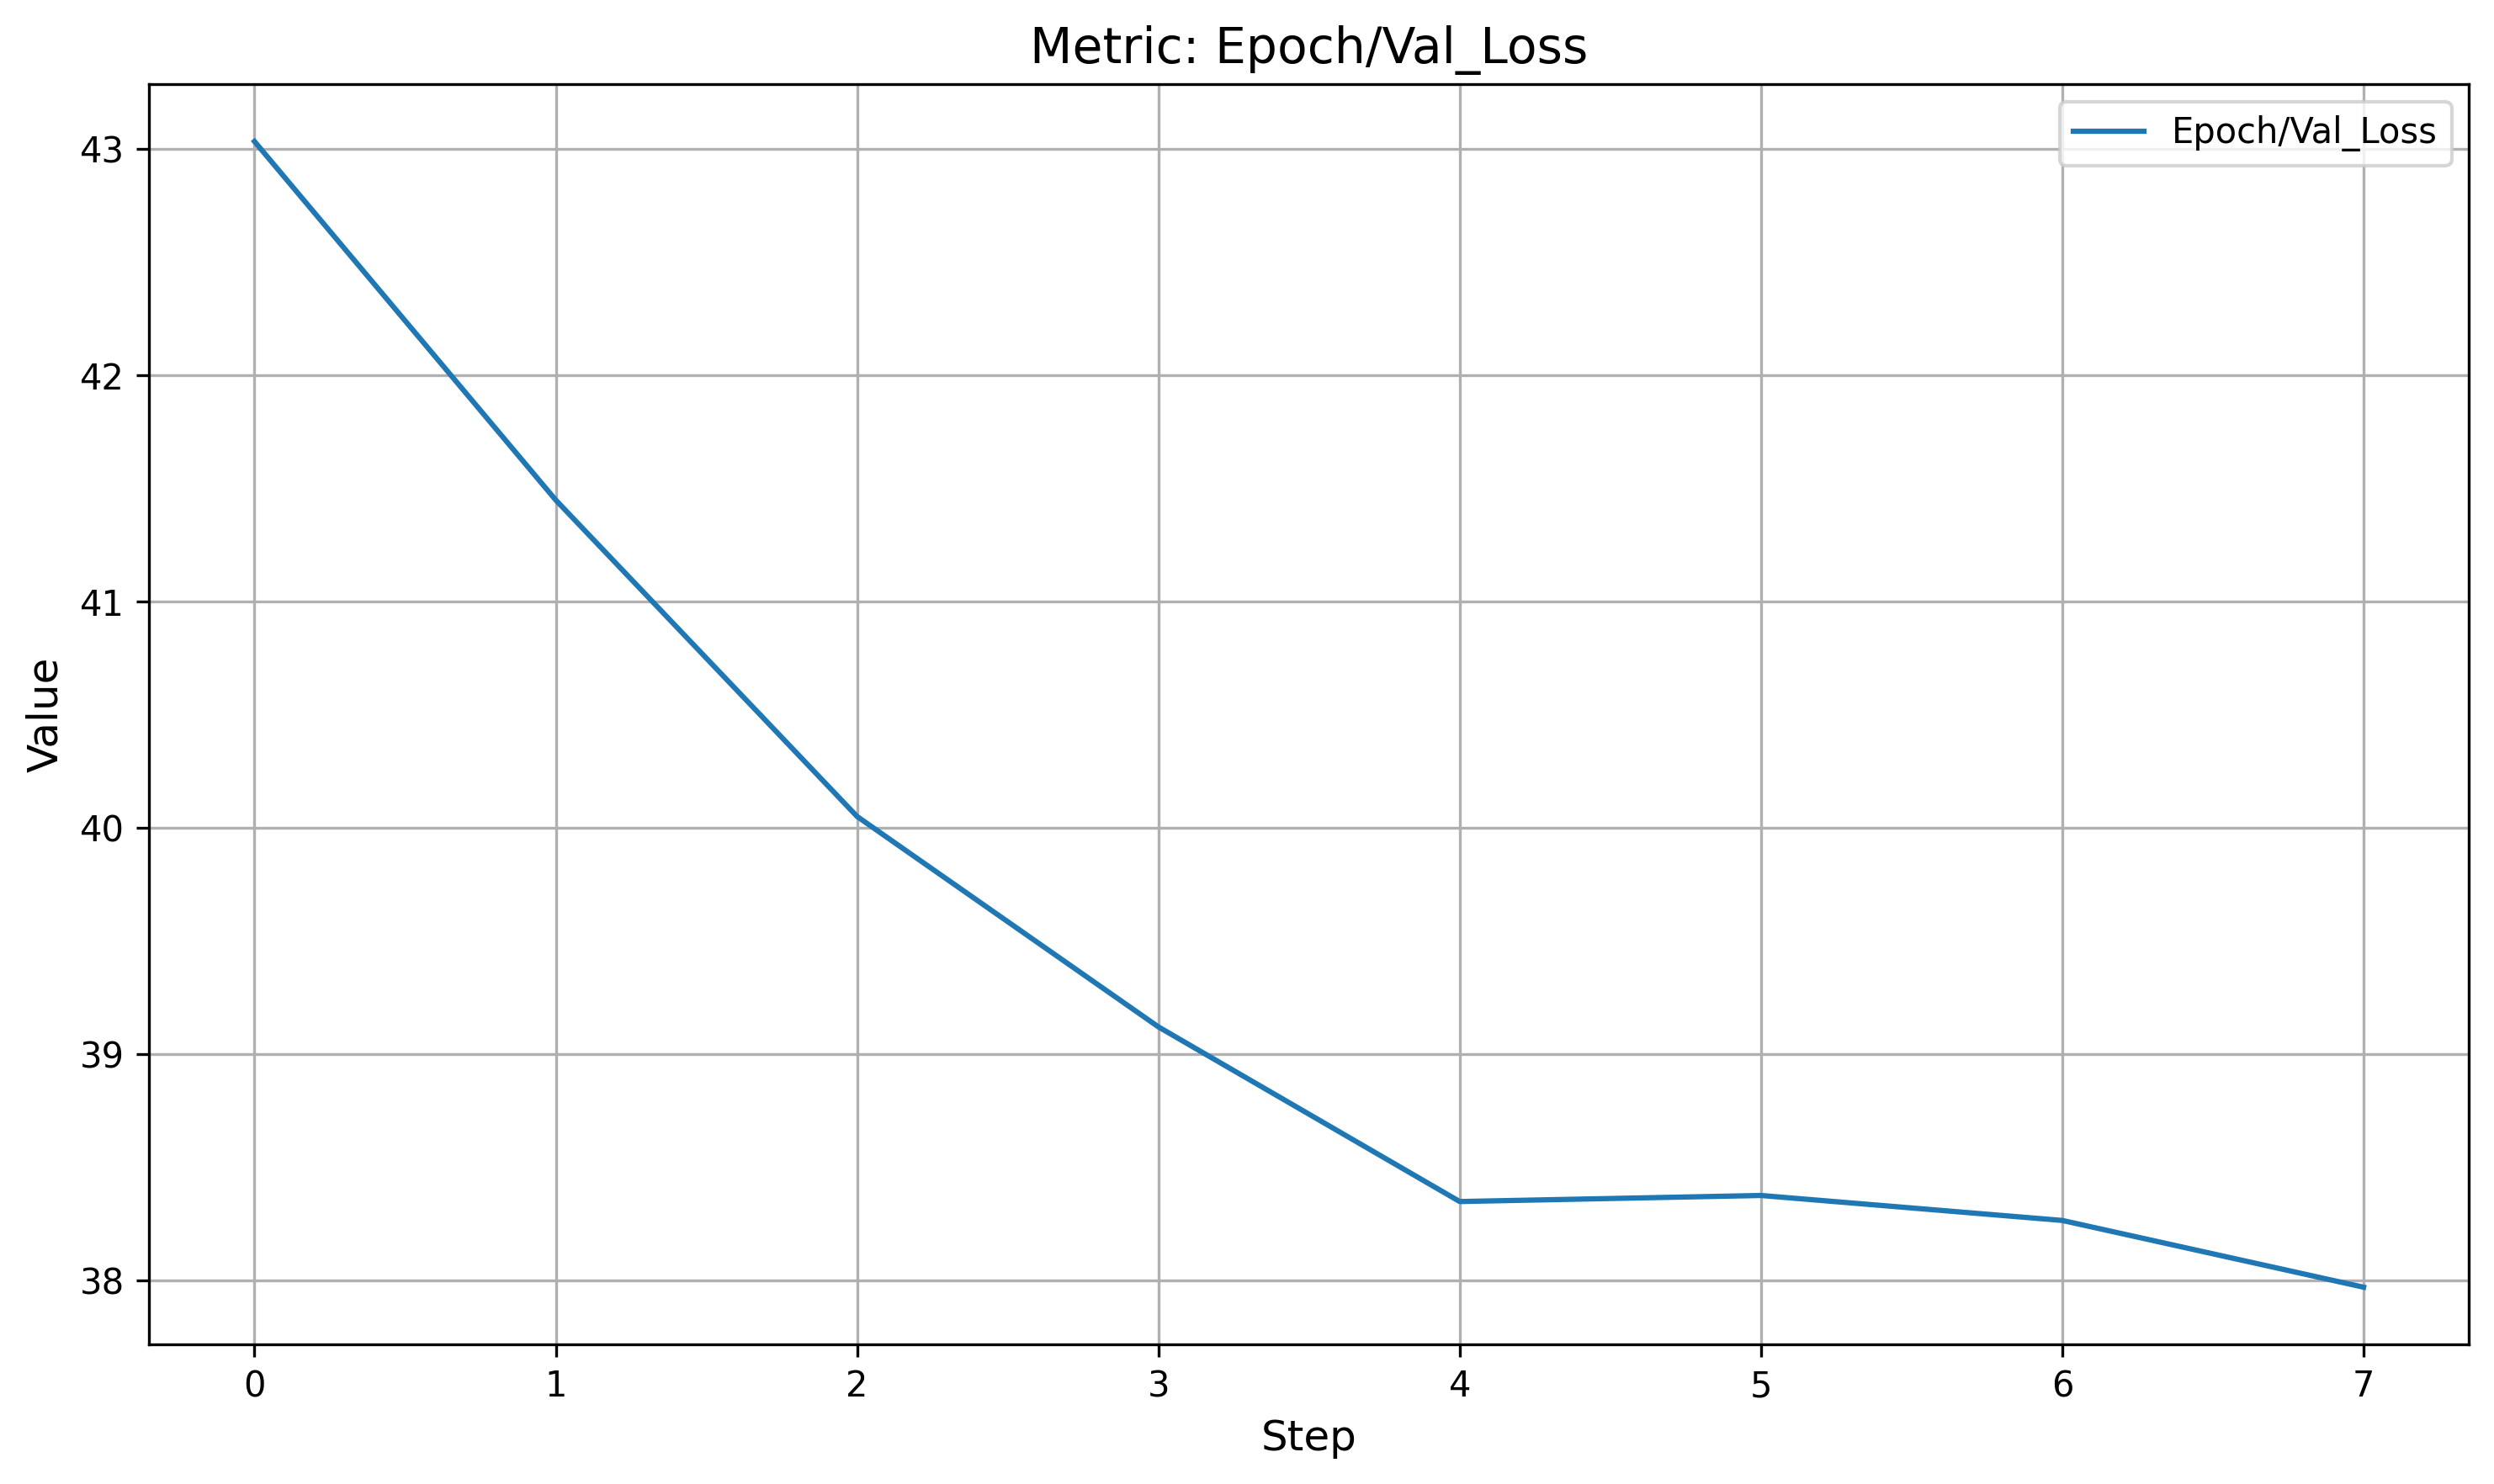
\includegraphics[width=\linewidth]{Images/ASR/Results/shaswot-graphs/EpochVal_Loss.png}
	\caption{Epoch Wise Validation Loss}
\end{figure}
Validation Loss (Figure 6-2) shows a similar downward trend, reaching 37.9 at epoch 7, with only minor fluctuations (e.g., a small uptick at epoch 5), suggesting good generalization without severe overfitting.

\begin{figure}[H]
	\centering
	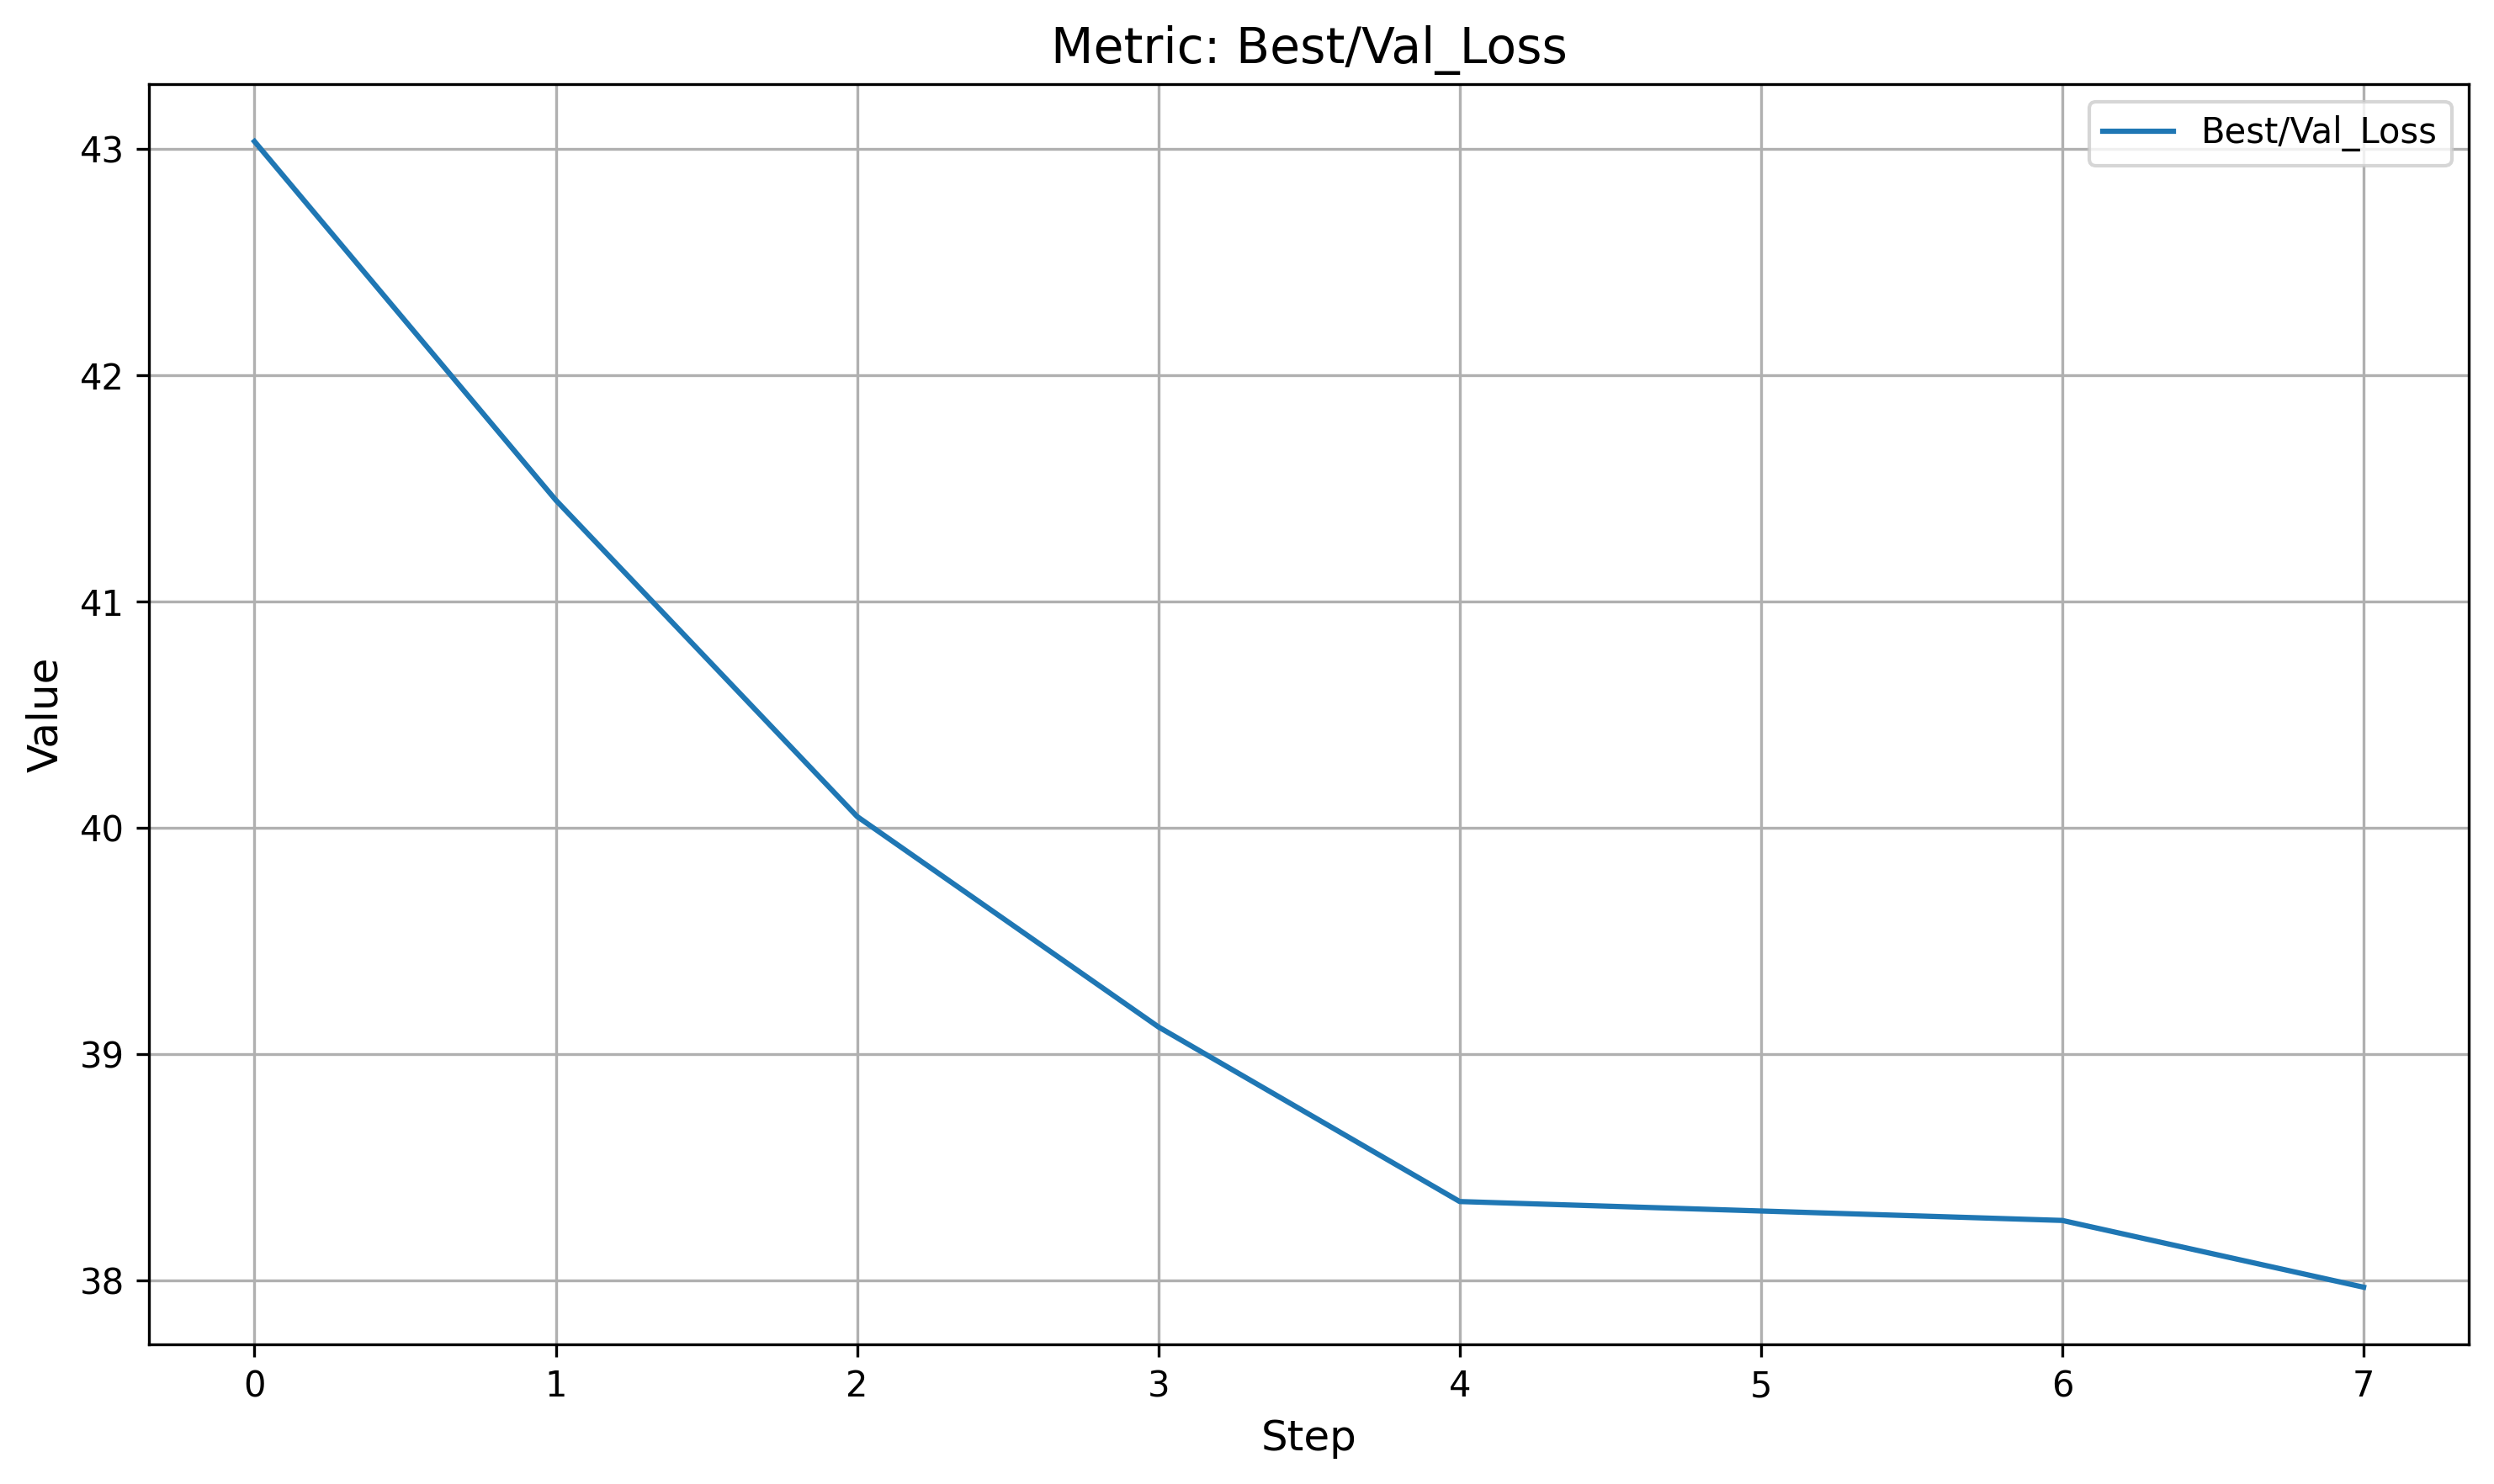
\includegraphics[width=\linewidth]{Images/ASR/Results/shaswot-graphs/BestVal_Loss.png}
	\caption{Best Validation Loss (Cumulative Minimum)}
\end{figure}
The Best Validation Loss (Figure 6-3) is monotonically non-increasing, confirming that the best checkpoint improves over time.
\begin{figure}[H]
	\centering
	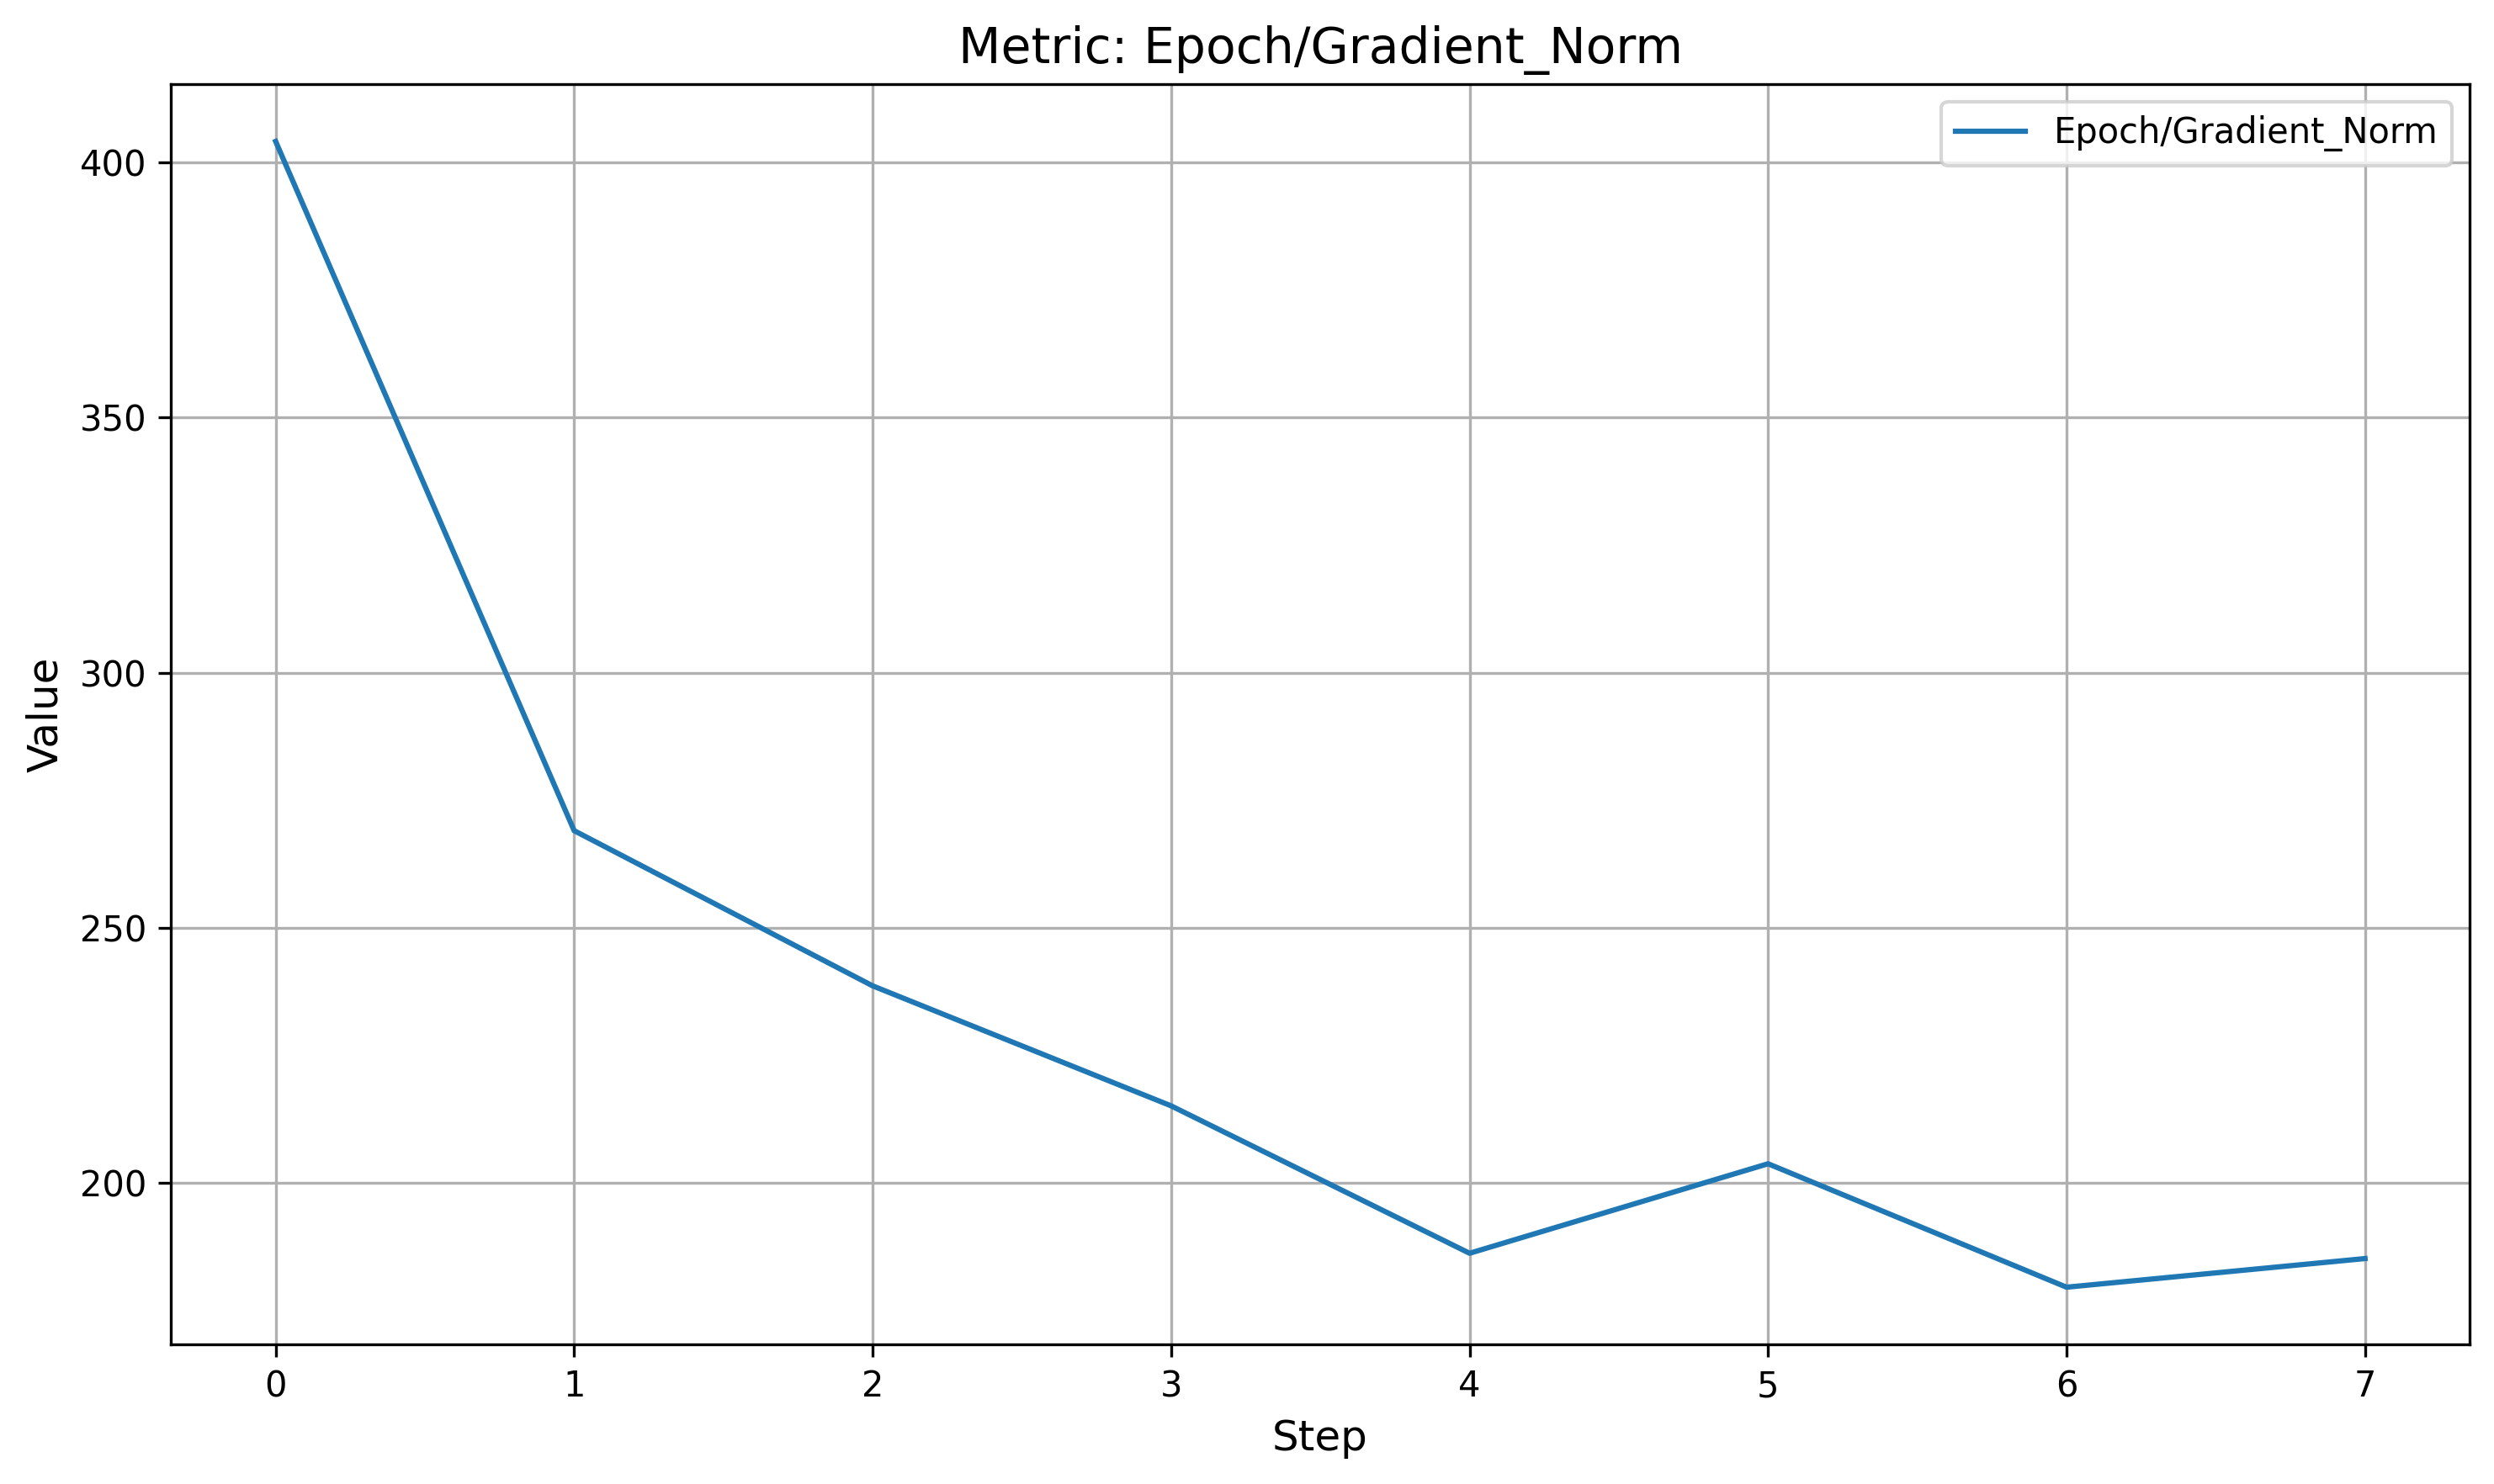
\includegraphics[width=\linewidth]{Images/ASR/Results/shaswot-graphs/EpochGradient_Norm.png}
	\caption{Gradient Norm per Epoch}
\end{figure}
The Gradient Norm (Figure 6-4) drops rapidly in early epochs and stabilizes around 180–185, signaling convergence and stable optimization. Collectively, these curves confirm a stable, well-behaved training process with no signs of divergence or instability.

\subsubsection{Dataset Preperation}
The Automatic Speech Recognition (ASR) datasets are usually based on 16 kHz mono audio due to the effective tradeoff between speech intelligibility and computational efficiency. The 16 kHz sampling frequency, which is based on the Nyquist theorem, retrieves the frequencies up to 8 kHz- the range that is most important to the human voice- without introducing the high-frequency data that is not necessary and beneficial to the recognition performance as offered by higher rates such as 44.1 kHz. Also, mono (single-channel) audio is common in ASR systems since recognition is based on phonemes and time, and not space or direction; downmixing stereo audio to mono reduces memory space by half, makes preprocessing and model construction much easier, and does not lose speech content that is important. Combined, these decisions help to cut down on data size and computational load to support faster and more efficient model training and inference without compromising accuracy.

OpenSLR54, Librispeech100 and OpenSLR12 hosted the dataset which contained the nepali and English audio dataset. The dataset was split into training set, validation set and test set in an 85:10:5 in a data of 10 hours to make sure that there is enough data to be used in the model learning and still have smaller portions to be used in the evaluation and tuning. In an effort of enhancing the strength of the ASR model, noise augmentation was done on each split separately. In particular, each subset consisted of 50\% samples that were randomly selected and noised with the environment. The four categories used in drawing the noise included crowd, construction, traffic, and wind to recreate the acoustic conditions in the real world. The individual clean audio samples were then randomly cross-mixed with a noise segment of these categories using a controlled SNR-based method, so as to guarantee a consistent noise intensity across the dataset. The rest half of the data were retained clean to have a balance in terms of noisy and noise free samples. Through this strategy, the model is able to learn the optimal and negative listening conditions, hence improving its generalization and performance in the real world implementation situations.

The majority of our data was obtained by OpenSLR. The files and its description are contained in manifest. Every sample has a distinct identifier, the audio file path, audio transcription, type of noise, signal to noise ratio in decibels, and dataset division (train, validation, or test). This format is easy to access and filter and is therefore appropriate to use in tasks such as speech recognition in dissimilar acoustic environments. For the purpose of testing independently, We used Fleurs dataset which contains about 2.28 hours of audio data with its transcript. The Fleurs dataset contains the clean audio file and the well-structured transcript for the nepali language. All the audio files here were embedded with noise using scripts with the SNR level similar to the training dataset and the dataset was used specifically for the purpose of testing our model.


\subsubsection{FastConformer-CTC-BPE}

\textbf{Model Architecture and PEFT Configuration}

The NVIDIA NeMo FastConformer-CTC-BPE model was used as the base automatic speech recognition system in the experiments. The model follows an encoder-decoder architecture that uses Connectionist Temporal Classification (CTC) loss for sequence-to-sequence mapping. The encoder is a Conformer-based model with approximately ~ 13 million parameters, while the decoder is a convolutional ASR decoder with 181,000 parameters. The total number of parameters in the base model is 13,204,721.

To achieve parameter-efficient fine-tuning, the NeMo adapter-based PEFT architecture was used. This approach is supported by NeMo as an alternative to LoRA for Conformer-based architectures. Adapter modules were inserted only into the encoder component, while all other parameters were kept frozen during training. Each adapter used a linear bottleneck architecture under the configurations shown in Table~\ref{tab:fastconformer_adapter}. This design reduced the number of trainable parameters to only 50,688, which corresponds to 0.3839\% of the total model parameters.

\begin{table}[H]
\caption{Adapter Configuration Parameters}
\label{tab:fastconformer_adapter}
\centering
\begin{tabular}{|l|l|}
\hline
\textbf{Parameter} & \textbf{Configuration Value} \\
\hline
Target Module & Encoder \\
Adapter Dimension & 8 \\
Adapter Dropout & 0.25 \\
Activation Function & Swish \\
Normalization Position & Pre-norm \\
Input Feature Size & 176 \\
Trainable Parameters & 50,688 \\
Trainable Percentage & 0.3839\% \\
\hline
\end{tabular}
\end{table}

\textbf{Dataset and Preprocessing}

Training was conducted on a custom English ASR dataset written in NeMo manifest format and stored as JSONL files. The dataset was divided into training, validation, and test subsets. All audio samples were processed at a sampling rate of 16,000 Hz. Duration filtering was applied to remove utterances shorter than 0.5 seconds and longer than 20 seconds.

The data loader used seven worker processes with pinned memory enabled to improve GPU data transfer efficiency. Silence trimming was disabled in order to preserve natural speech characteristics. Table~\ref{tab:fastconformer_dataset} presents the statistical distribution of the dataset splits.

\begin{table}[H]
\caption{Dataset Split Statistics}
\label{tab:fastconformer_dataset}
\centering
\begin{tabular}{|l|l|l|l|}
\hline
\textbf{Split} & \textbf{Samples} & \textbf{Duration} & \textbf{Average Words} \\
\hline
Train & 4,859 & 17.03 hours & 35.26 \\
Validation & 571 & 1.99 hours & 35.26 \\
Test & 287 & 0.98 hours & 35.10 \\
\hline
\end{tabular}
\end{table}

\textbf{Training Configuration}

Training was performed using PyTorch Lightning together with the NeMo toolkit. Optimization was carried out using AdamW with decoupled weight decay. A cosine annealing scheduler was used to control the learning rate, together with a warmup phase to stabilize the initial training dynamics. Bfloat16 mixed precision training was enabled to reduce memory usage and accelerate computation on the available GPU hardware. The training hyperparameters are summarized in Table~\ref{tab:fastconformer_train}.

\begin{table}[H]
\caption{Training Hyperparameters}
\label{tab:fastconformer_train}
\centering
\begin{tabular}{|l|l|}
\hline
\textbf{Parameter} & \textbf{Value} \\
\hline
Maximum Epochs & 15 \\
Batch Size & 32 \\
Gradient Accumulation Steps & 2 \\
Learning Rate & $1\times10^{-4}$ \\
Minimum Learning Rate & $1\times10^{-6}$ \\
Weight Decay & $5\times10^{-2}$ \\
Adam Betas & (0.9, 0.98) \\
Warmup Ratio & 0.1 \\
Gradient Clipping & 1.0 \\
Precision & bf-16 mixed\\
Learning Rate Scheduler & Cosine Annealing \\
\hline
\end{tabular}
\end{table}

\textbf{Data Augmentation}

SpecAugment was applied during training to improve model robustness against acoustic variability. This augmentation strategy helps the model generalize better to unseen acoustic conditions by masking selected regions of the spectrogram. The frequency and time masking configurations are shown in Table~\ref{tab:fastconformer_aug}.

\begin{table}[H]
\caption{Data Augmentation Parameters}
\label{tab:fastconformer_aug}
\centering
\begin{tabular}{|l|l|l|}
\hline
\textbf{Augmentation Type} & \textbf{Count} & \textbf{Maximum Width} \\
\hline
Frequency Masks & 2 & 15 frequency bins \\
Time Masks & 6 & 30 time steps \\
\hline
\end{tabular}
\end{table}

\textbf{Regularization and Checkpointing}

Early stopping was based on validation Word Error Rate (WER) as the monitoring metric. Model checkpoints were saved at regular intervals, and the best-performing checkpoint was retained according to validation performance. This strategy helped reduce overfitting and ensured that the best model weights were preserved for final evaluation. The checkpointing and early stopping criteria are given in Table~\ref{tab:fastconformer_ckpt}.

\begin{table}[H]
\caption{Checkpoint and Early Stopping Configuration}
\label{tab:fastconformer_ckpt}
\centering
\begin{tabular}{|l|l|}
\hline
\textbf{Configuration} & \textbf{Value} \\
\hline
Monitor Metric & Validation WER \\
Mode & Minimization \\
Patience & 5 epochs \\
Minimum Delta & 0.0 \\
Save Top K & 1 \\
Checkpoint Frequency & Every 1 epoch \\
\hline
\end{tabular}
\end{table}

\textbf{Evaluation Metrics}

Standard ASR evaluation metrics were used to measure model performance. Word Error Rate (WER) was computed using Levenshtein distance between reference and hypothesis word sequences. Character Error Rate (CER) was calculated using character-level Levenshtein distance. These metrics were evaluated both through the PyTorch Lightning evaluation pipeline and through offline transcription on the validation and test sets. Whitespace was preserved during text normalization so that both metrics could be computed consistently. The model achieved a best validation WER of 3.240\%.

\textbf{Software and Hardware Environment}

A fixed software stack was used to ensure reproducibility of the implementation. All experiments were conducted on Google Colab using an NVIDIA Tesla T4 GPU. Deterministic training was enabled in warn-only mode to account for non-deterministic GPU CTC backward operations while maintaining reproducibility wherever possible. A random seed of 42 was used throughout the experiments. The software and hardware specifications are provided in Table~\ref{tab:fastconformer_env}.

\begin{table}[H]
\caption{Software and Hardware Configuration}
\label{tab:fastconformer_env}
\centering
\begin{tabular}{|l|l|}
\hline
\textbf{Component} & \textbf{Version / Specification} \\
\hline
NVIDIA NeMo Toolkit & 2.4.0 \\
PyTorch Lightning & $\geq$ 2.2.0, $<$ 2.6.0 \\
Python & 3.12 \\
CUDA & 12.8 \\
NumPy & 1.26.4 \\
GPU Accelerator & NVIDIA Tesla T4 \\
Random Seed & 42 \\
\hline
\end{tabular}
\end{table}

\textbf{Model Export and Checkpointing}

After training, the best model checkpoint was exported in multiple formats to support different deployment scenarios. The complete model was saved in NeMo format with full model weights for direct deployment. In addition, the adapter weights were saved separately in PyTorch format, containing only the trainable adapter parameters for efficient storage and transfer. This dual-export strategy supports both full-model deployment and adapter-only fine-tuning in resource-constrained environments.

\subsubsection{Implementation Details for Indic Conformer}

\textbf{Model Architecture and Configuration}

The automatic speech recognition system was built using the IndicConformer \texttt{stt\_ne\_conformer\_ctc\_rnnt\_large} variant. This model uses a hybrid loss function that combines Connectionist Temporal Classification (CTC) and Recurrent Neural Network Transducer (RNNT) objectives, allowing it to benefit from both alignment-free and sequence-to-sequence training paradigms.

The architecture consists of a Conformer-based encoder, an RNNT decoder, a joint network, and an additional CTC decoder head. The model uses a SentencePiece tokenizer with a vocabulary of 5,632 tokens, derived from 256 tokens per language unit. Unlike the FastConformer-CTC-BPE setup, all model parameters were fully fine-tuned, resulting in approximately 129 million trainable parameters. Table~\ref{tab:indic_model} summarizes the main architectural components and their parameter distribution.

\begin{table}[H]
\caption{Model Components and Parameter Distribution}
\label{tab:indic_model}
\centering
\begin{tabular}{|l|l|l|l|}
\hline
\textbf{Component} & \textbf{Module Type} & \textbf{Parameters} & \textbf{Mode} \\
\hline
Preprocessor & AudioToMelSpectrogramPreprocessor & 0 & Train \\
Encoder & ConformerEncoder & 115 M & Train \\
Decoder & RNNTDecoder & 6.9 M & Train \\
Joint Network & RNNTJoint & 4.4 M & Train \\
CTC Decoder & ConvASRDecoder & 2.9 M & Train \\
Loss Functions & RNNTLoss, CTCLoss & 0 & Train \\
\textbf{Total} & -- & 129 M & Train \\
\hline
\end{tabular}
\end{table}

\textbf{Dataset and Preprocessing Pipeline}

The experiments were conducted on a Nepali speech dataset split into training and validation subsets. All audio files were standardized to mono-channel format with a sampling rate of 16,000 Hz. Manifest files were normalized to ensure consistency across transcription-related fields such as \texttt{text}, and \texttt{transcript}, which were mapped to a common format.

No additional audio resampling was applied during fine-tuning, and silence trimming was disabled to preserve natural speech characteristics. Table~\ref{tab:indic_dataset} presents the dataset statistics, including sample counts and duration.

\begin{table}[H]
\caption{Dataset Duration Statistics}
\label{tab:indic_dataset}
\centering
\begin{tabular}{|l|l|l|l|}
\hline
\textbf{Split} & \textbf{Sample Count} & \textbf{Duration (Hours)} & \textbf{Average Duration (Seconds)} \\
\hline
Training & 15,820 & 15.59 & 3.55 \\
Validation & 3,955 & 3.82 & 3.48 \\
\hline
\end{tabular}
\end{table}

\textbf{Training Hyperparameters and Optimization}

The model was fine-tuned using PyTorch Lightning together with the AI4Bharat NeMo fork. AdamW with decoupled weight decay was used as the optimizer. The learning rate schedule followed a WarmupAnnealing strategy with 500 warmup steps followed by annealing. Training was conducted for up to 15 epochs with a batch size of 16 samples per step.

Gradient clipping with a value of 1.0 was applied to stabilize optimization. Early stopping with a patience of 3 epochs was used based on validation WER to reduce overfitting. The full training configuration is given in Table~\ref{tab:indic_train}.

\begin{table}[H]
\caption{Training Hyperparameters}
\label{tab:indic_train}
\centering
\begin{tabular}{|l|l|}
\hline
\textbf{Hyperparameter} & \textbf{Value} \\
\hline
Maximum Epochs & 15 \\
Training Batch Size & 32 \\
Evaluation Batch Size & 64 \\
Gradient Accumulation & 1 \\
Learning Rate & $5\times10^{-5}$ \\
Weight Decay & $1\times10^{-3}$ \\
Warmup Steps & 1000 \\
Gradient Clipping & 1.0 \\
Early Stopping Patience & 5 \\
Early Stopping Min Delta & 0.001 \\
Checkpoint Save Top K & 2 \\
Validation Frequency & Every 1 Epochs \\
\hline
\end{tabular}
\end{table}

\textbf{Regularization and Augmentation}

SpecAugment was used during training to improve robustness against noise and acoustic variability. The implementation used a Numba CUDA kernel for efficient spectrogram masking. The augmentation strategy included both frequency masking and time masking of the input spectrograms.

Brain floating point 16bit (bf16-mixed) was also enabled to reduce memory consumption and speed up computation. Table~\ref{tab:indic_runtime} shows the runtime and optimization settings.

\begin{table}[H]
\caption{Runtime and Optimization Settings}
\label{tab:indic_runtime}
\centering
\begin{tabular}{|l|l|}
\hline
\textbf{Configuration} & \textbf{Setting} \\
\hline
Spectrogram Augmentation & Enabled \\
Augmentation Kernel & Numba CUDA \\
Precision & bf16-mixed\\
Matrix Multiplication Precision & Medium \\
CuDNN Benchmark & Enabled \\
\hline
\end{tabular}
\end{table}

\textbf{Hardware and Software Environment}

All experiments were carried out in Google Colab with high-performance GPU acceleration. The software stack included the AI4Bharat fork of NVIDIA NeMo, patched for compatibility with NumPy 2.x runtimes. Particular attention was given to version compatibility for PyTorch and PyTorch Lightning to ensure reproducibility. The system specifications are shown in Table~\ref{tab:indic_env}.

\begin{table}[H]
\caption{System and Software Specifications}
\label{tab:indic_env}
\centering
\begin{tabular}{|l|l|}
\hline
\textbf{Component} & \textbf{Specification} \\
\hline
GPU & NVIDIA A100-SXM4-80GB \\
CUDA Version & 12.8 \\
PyTorch Version & 2.10.0+cu128 \\
PyTorch Lightning & 2.6.1 \\
NeMo Version & 1.23.0rc0 \\
Python Version & 3.12 \\
NumPy Version & 2.0.2 \\
\hline
\end{tabular}
\end{table}

\textbf{Evaluation Metrics and Checkpointing}

Validation Word Error Rate (WER) and Character Error Rate (CER) were used as the primary performance metrics and were computed every second epoch. The training loop also tracked the individual CTC and RNNT loss components to monitor convergence of both objectives.

Model checkpoints were selected based on the lowest validation WER, and the top two checkpoints were retained for final evaluation. The monitored metrics included training loss, validation loss, and the corresponding CTC and RNNT loss components. The evaluation and checkpointing setup is summarized in Table~\ref{tab:indic_eval}.

\begin{table}[H]
\caption{Training and Evaluation Metrics}
\label{tab:indic_eval}
\centering
\begin{tabular}{|l|l|l|}
\hline
\textbf{Metric} & \textbf{Description} & \textbf{Monitoring Frequency} \\
\hline
Validation WER & Primary Optimization Metric & Every 1 Epoch \\
Validation CER & Secondary Accuracy Metric & Every 1 Epoch \\
Training Loss & Combined CTC and RNNT Loss & Every 5 Steps \\
Validation Loss & Combined CTC and RNNT Loss & Every 1 Epoch \\
Checkpoint Monitor & val\_wer\_eval & Every 1 Epoch \\
Checkpoint Mode & Minimization & Every 1 Epoch \\
Early Stopping & Patience = 5, Min Delta = 0.001 & Checked Every 1 Epoch \\
Checkpoint Saving & Top 2 Model Saved & Based on Validation Metric \\
\hline
\end{tabular}
\end{table}

\subsubsection{Model Exporting and Quantization for Indic Conformer}

The fine-tuned IndicConformer Hybrid CTC/RNNT Large model, containing 129 million parameters, was converted to the Open Neural Network Exchange (ONNX) format using a conversion pipeline based on the NVIDIA NeMo framework. After export, post-training quantization was applied to reduce storage requirements and improve deployment efficiency. The export configuration and quantization strategy are described below.

\textbf{Model Export Configuration (NeMo to ONNX)}

The AI4Bharat fork of NVIDIA NeMo (branch \texttt{nemo-v2}) was used to export the model. Because of the architectural complexity of the Conformer encoder, especially the \texttt{rel\_shift} attention mechanism, the legacy TorchScript-based ONNX exporter was used instead of the newer PyTorch Dynamo exporter in order to avoid symbolic shape-related errors. During export, the decoder head was isolated to ensure compatibility with standard inference engines.

\begin{table}[H]
\caption{Model Export Configuration}
\centering
\begin{tabular}{|l|l|}
\hline
\textbf{Configuration Parameter} & \textbf{Setting / Value} \\
\hline
Source Framework & NVIDIA NeMo (AI4Bharat nemo-v2) \\
Model Architecture & EncDecHybridRNNTCTCBPEModel \\
Export Format & ONNX  \\
Decoder Strategy & CTC \\
Input Tensor & \texttt{audio\_signal} (float32), \texttt{length} (int64) \\
Output Tensor & \texttt{logprobs} (float32) \\
Export Device & CUDA \\
\hline
\end{tabular}
\end{table}

\textbf{Quantization Strategy}

To make the model suitable for deployment in resource-constrained environments, dynamic post-training quantization was applied to the exported FP32 ONNX model. This method converts model weights from floating point to integer representation without requiring a calibration dataset. As a result, the deployment pipeline remains simple while still providing substantial storage savings with acceptable accuracy retention.

\begin{table}[H]
\caption{Quantization Configuration}
\centering
\begin{tabular}{|l|l|}
\hline
\textbf{Quantization Parameter} & \textbf{Setting / Value} \\
\hline
Quantization Library & onnxruntime.quantization \\
Method & Dynamic Quantization  \\
Weight Precision & INT8 \\
Activation Precision & FP32 \\
\hline
\end{tabular}
\end{table}

\textbf{Storage Optimization Results}

The quantization pipeline resulted in a significant reduction in model storage size. Table~\ref{tab:quant_result} compares the original exported model with the quantized version.

\begin{table}[H]
\caption{Model Size Comparison Before and After Quantization}
\label{tab:quant_result}
\centering
\begin{tabular}{|l|l|l|l|}
\hline
\textbf{Model Stage} & \textbf{Precision} & \textbf{File Size (MB)} & \textbf{Size Reduction (\%)} \\
\hline
Indic Conformer & FP32 & 493.05 & --- \\
Exported ONNX & FP32 & 470.22 & 4.6\% \\
Quantized ONNX & INT8 & 133.94 & 71.51\% \\
\hline
\end{tabular}
\end{table}

The quantized implementation reduced the model footprint by approximately 71.5\%, making it more suitable for deployment on edge devices and in environments with limited storage capacity. At the same time, the original inference logic of the architecture was preserved through ONNX Runtime execution.